\chapter{HCI Trial Charts (Study 14)}
\label{appendix:hci-trial-charts}

This appendix presents the visual representations of Study~14 (Section~\ref{subsec:hci-trial-protocol}).
Refer to Table~\ref{tab:hci-trial-results} for the raw data.

\begin{figure}[htbp]
    \centering
    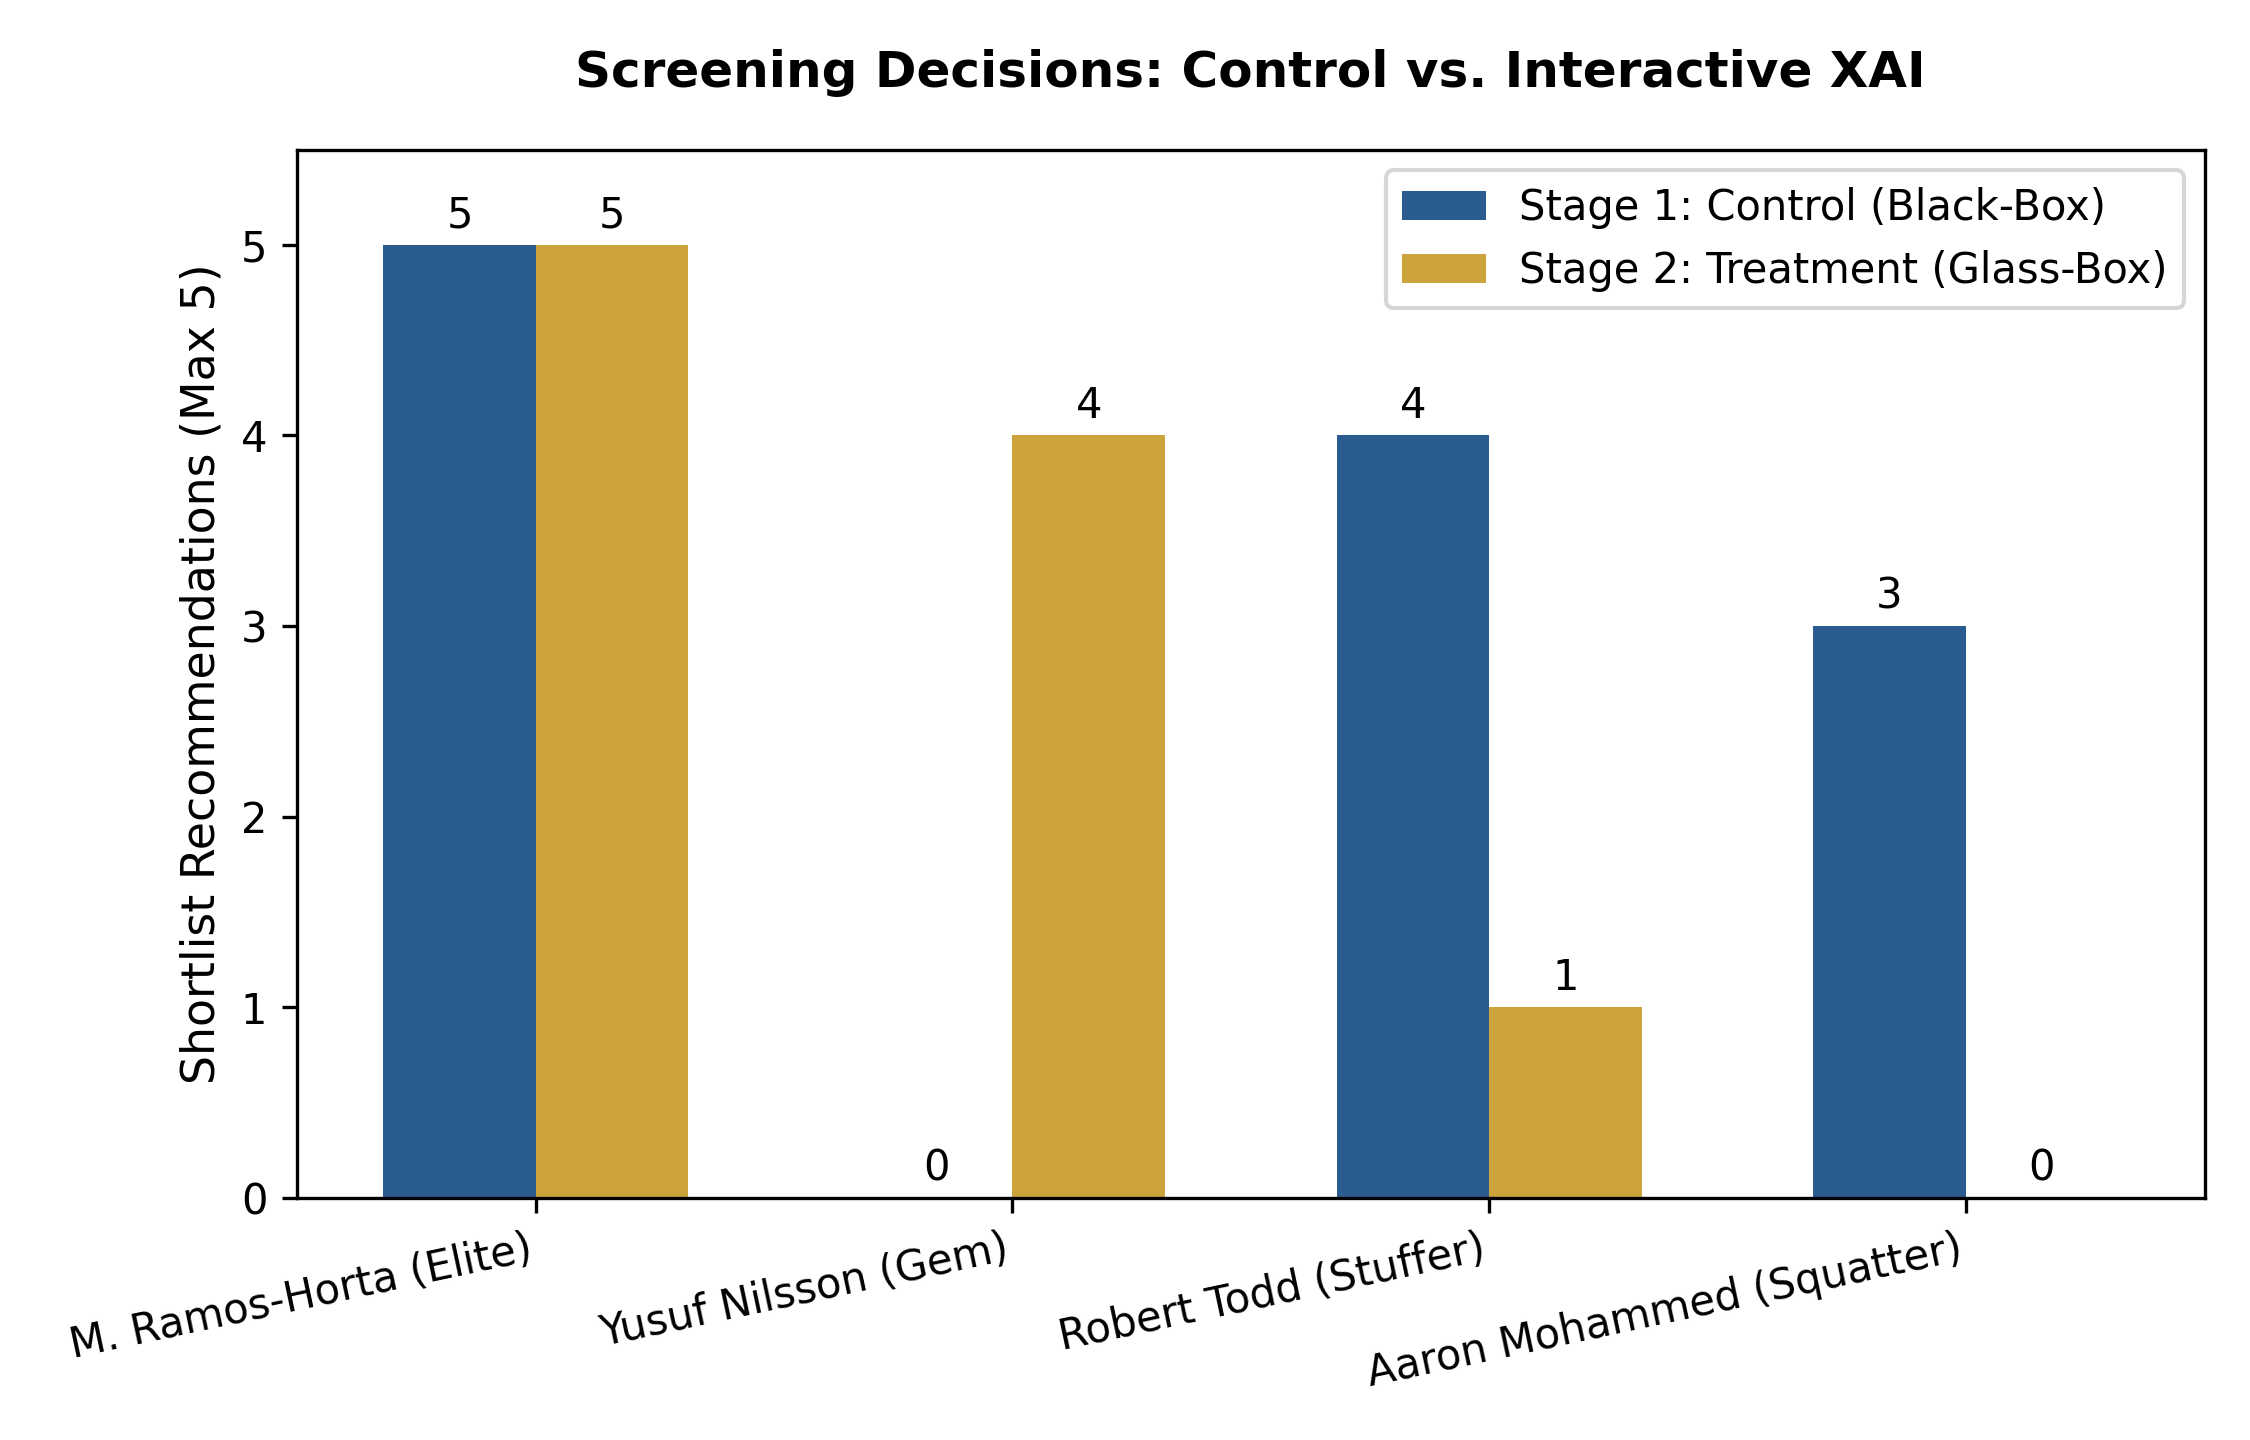
\includegraphics[width=0.92\textwidth]{../evaluation/14-hci_trial/output/hci_decision_reversals.png}
    \caption[Study~14: Decision reversal rates]{Study~14: Graphical representation of the decision shortlist
    recommendations pre/post Glass-Box exposure. Table data, as well as reasonings behind the results
    are provided in Table~\ref{tab:hci-trial-results}.}
    \label{fig:hci-decision-reversals}
\end{figure}

\begin{figure}[htbp]
    \centering
    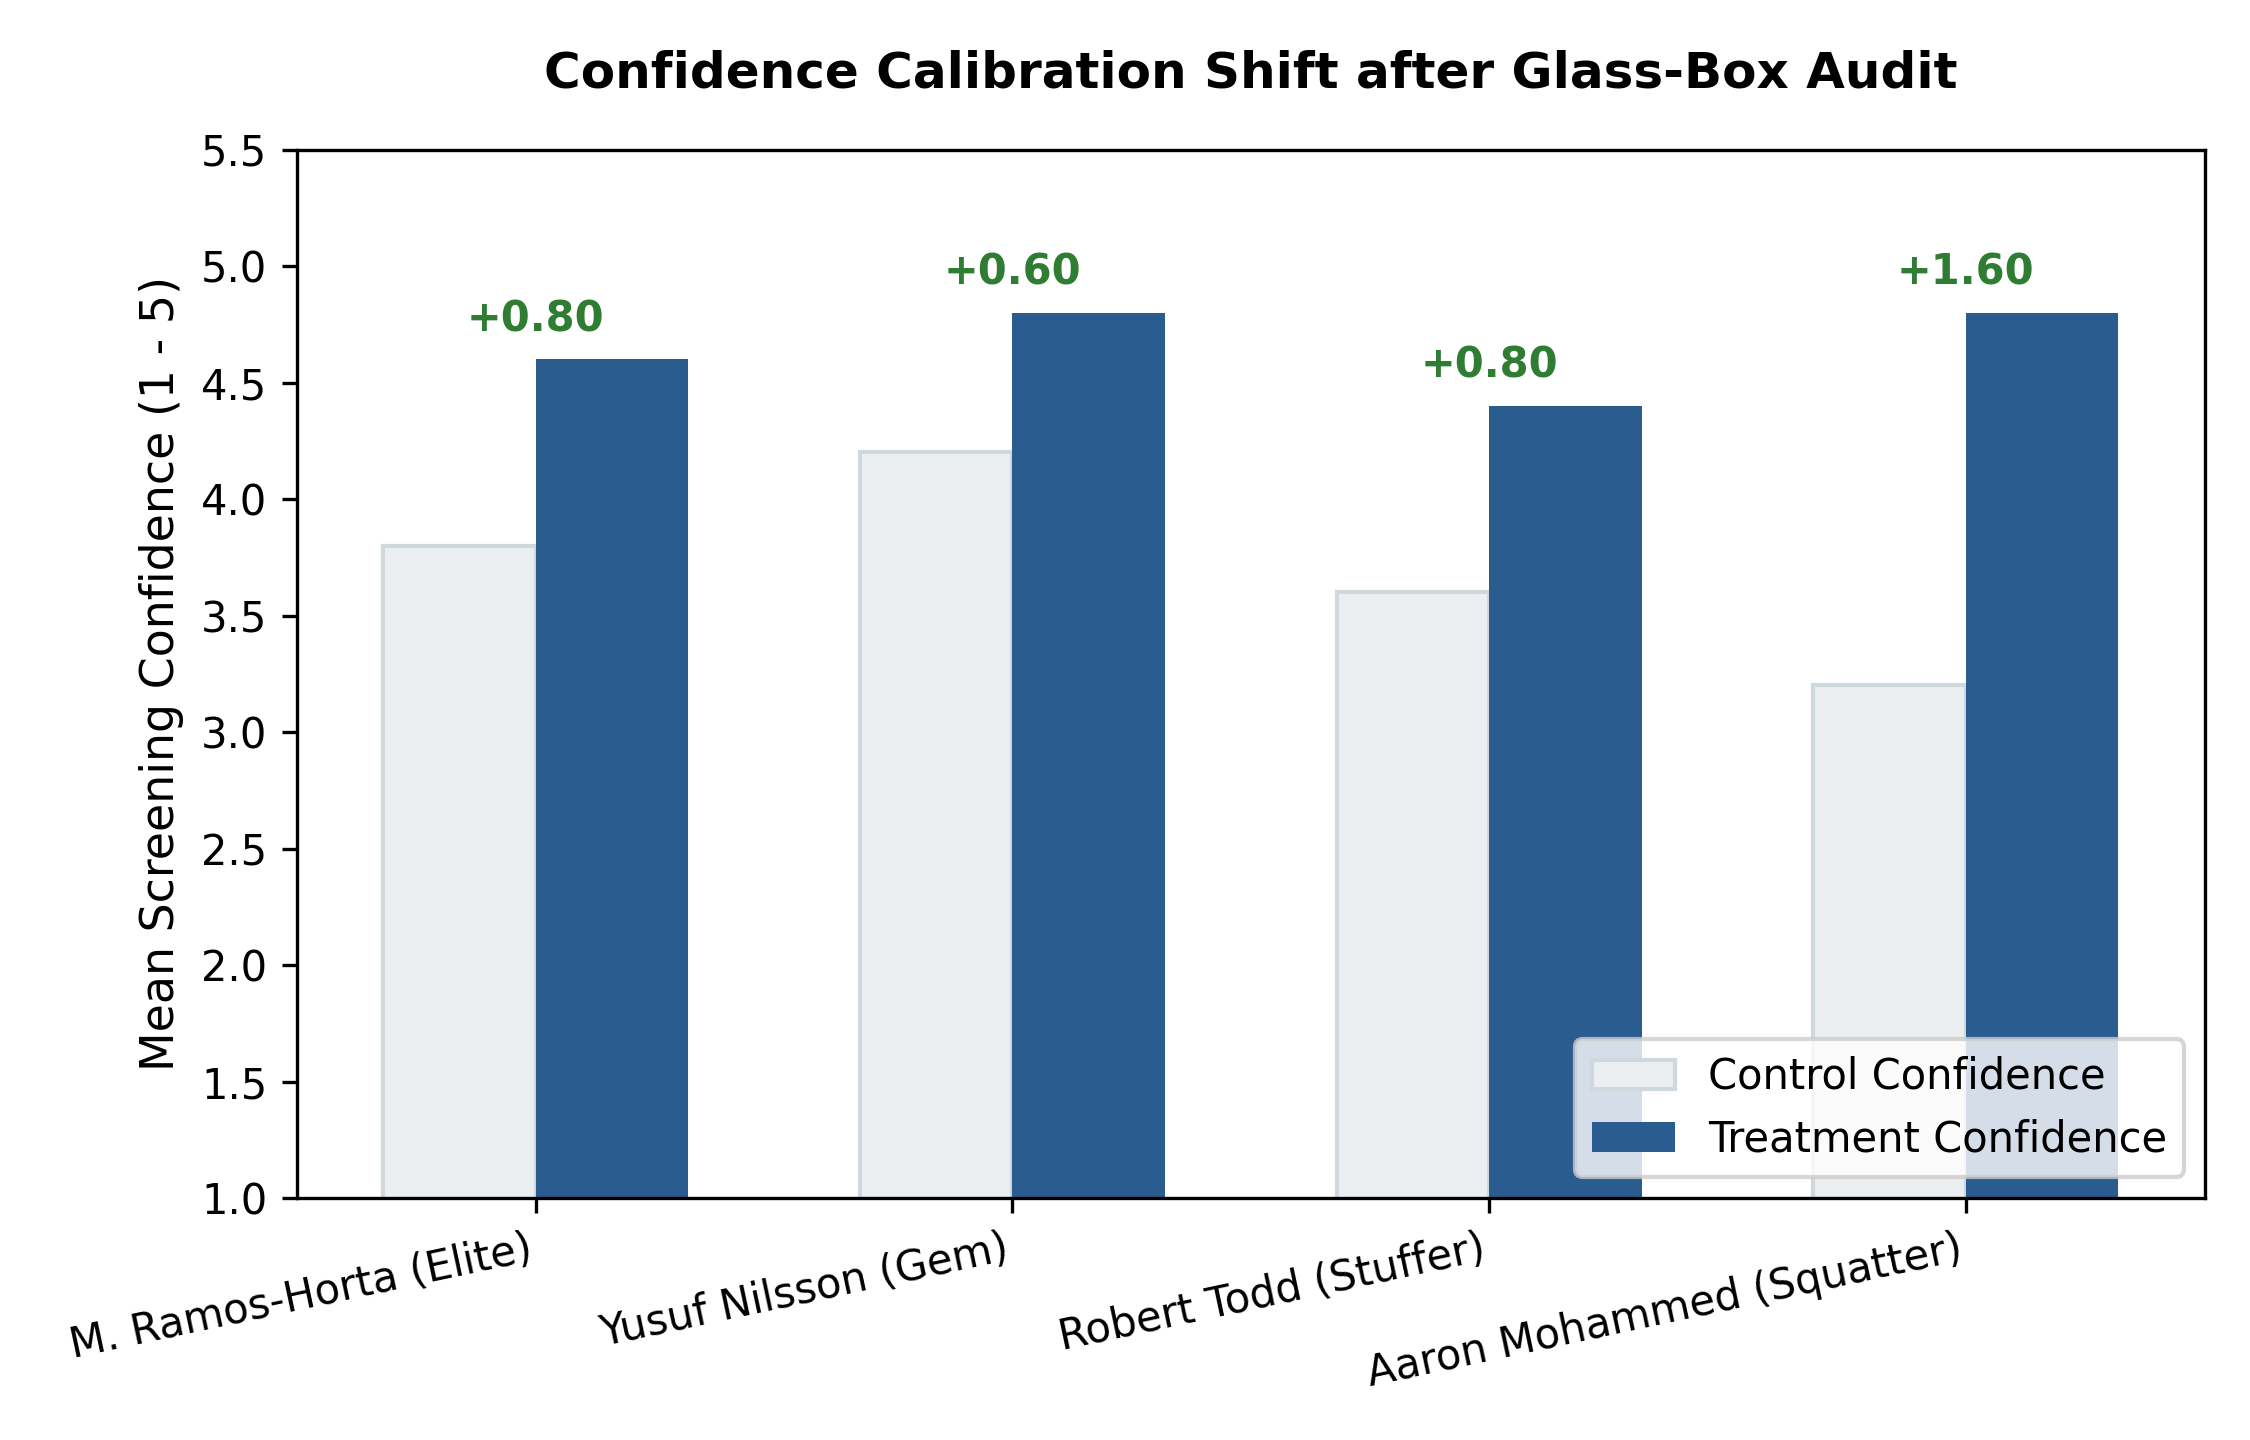
\includegraphics[width=0.92\textwidth]{../evaluation/14-hci_trial/output/hci_confidence_calibration.png}
    \caption[Study~14: Confidence calibration]{Study~14: Bar chart representation of the confidence callibration
    shifts after the glass box audit. Note that this is separated per-candidate, and we apply a mean of the evaluator
    confidence ratings to get a mean confidence rating for each candidate. We use a 5-point Likert scale
    to measure the confidence of the recruiter in their decision pre/post Glass-Box exposure, not taking into 
    account whether there was a decision reversal or not in this visualisation.}
    \label{fig:hci-confidence-calibration}
\end{figure}

\begin{figure}[htbp]
    \centering
    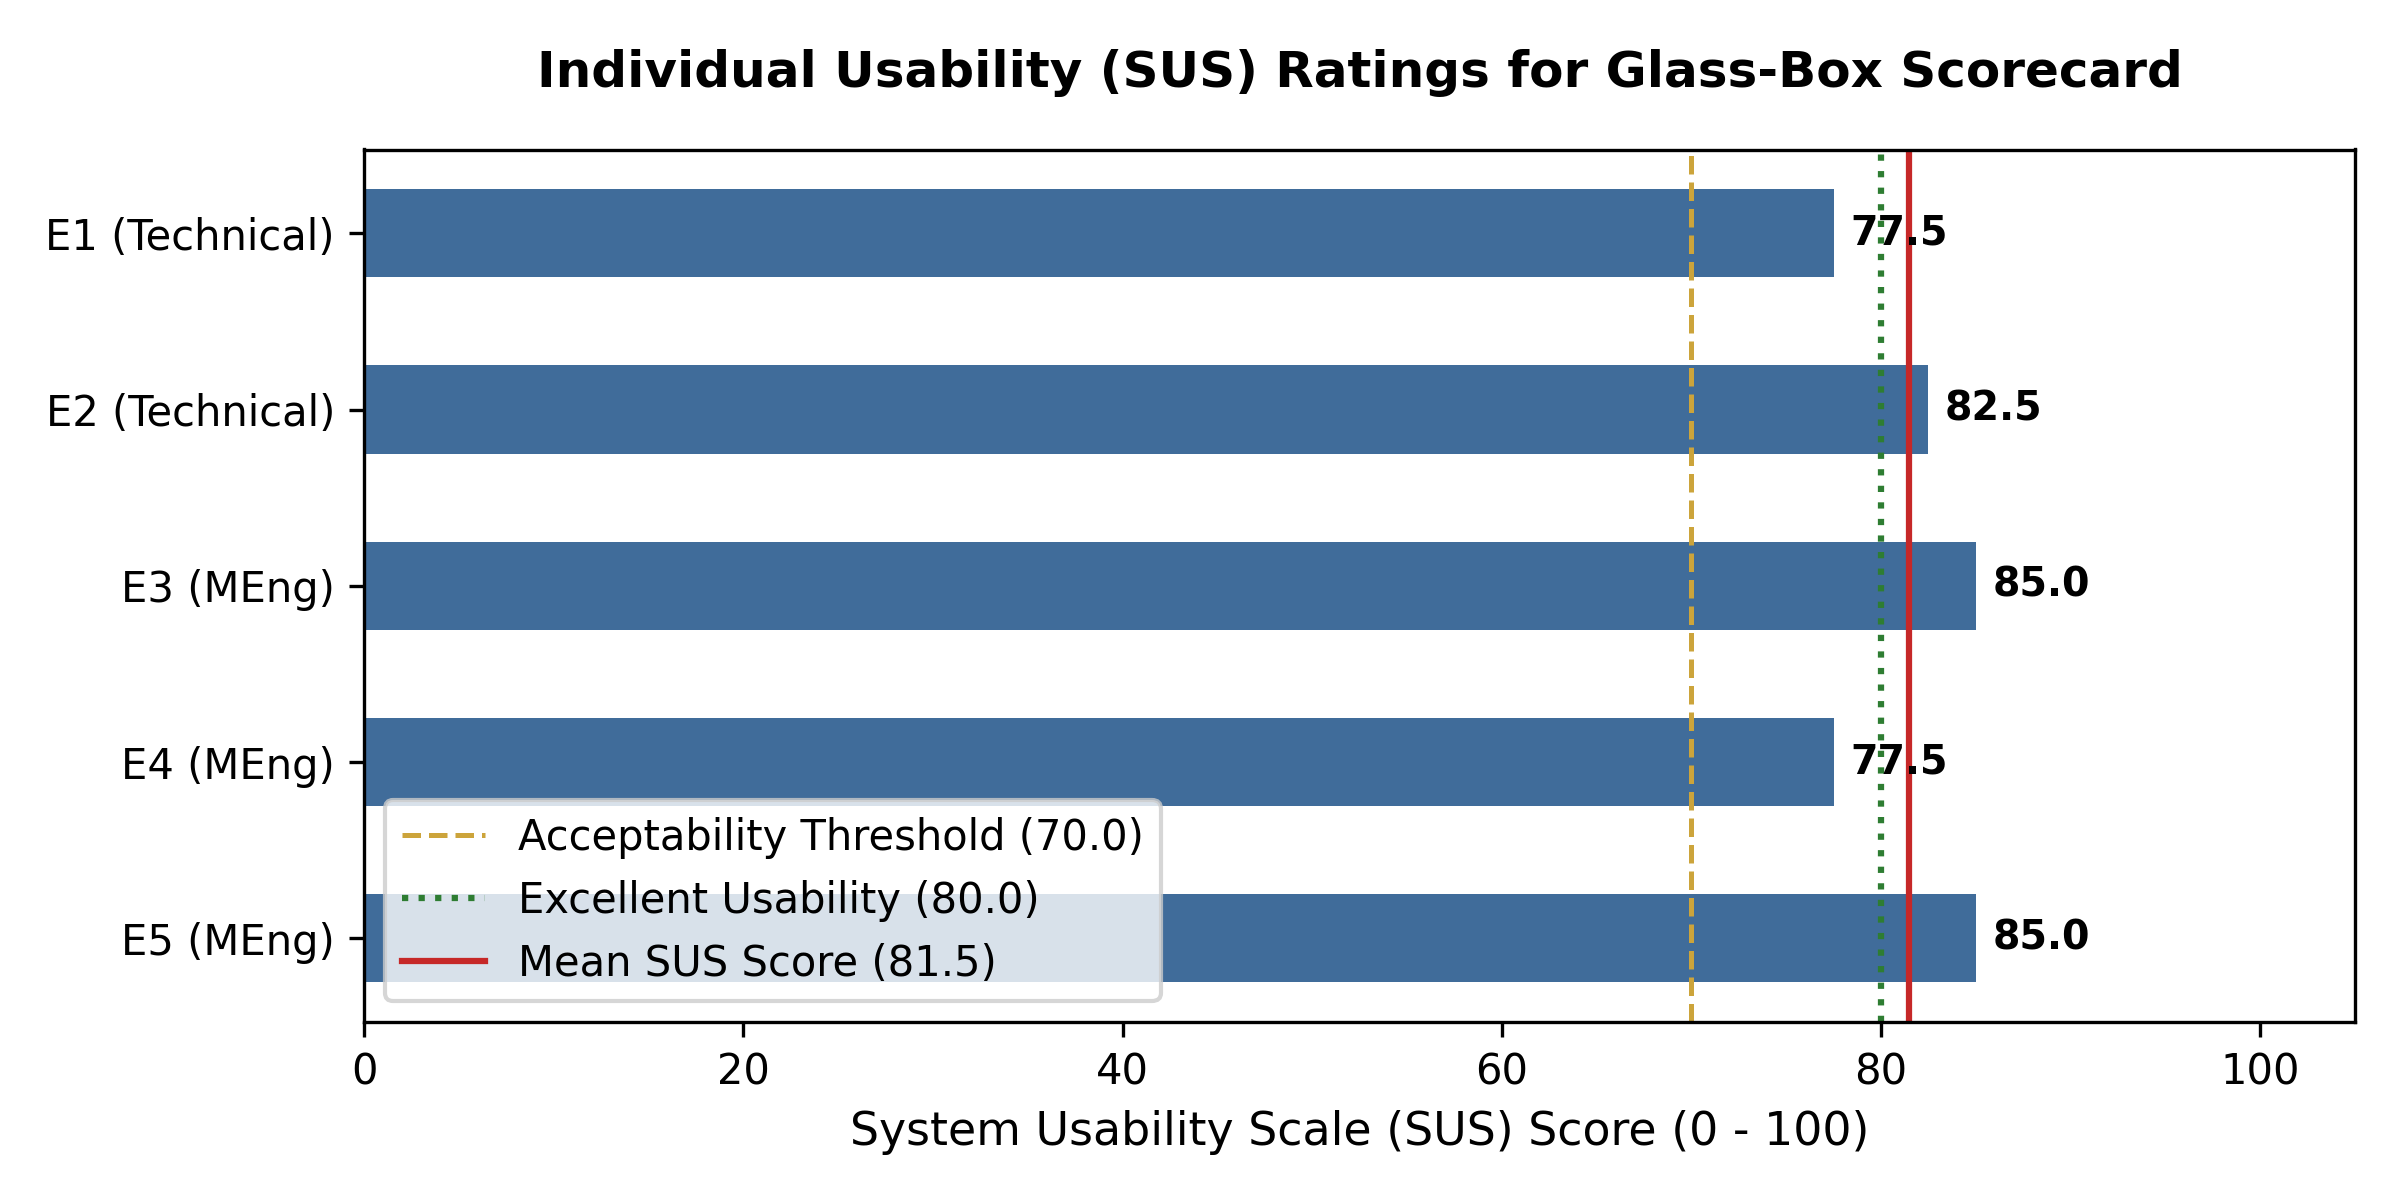
\includegraphics[width=0.85\textwidth]{../evaluation/14-hci_trial/output/hci_sus_distribution.png}
    \caption[Study~14: SUS scores by evaluator]{Study~14: Bar chart representation of the SUS scores by evaluator.
    A total of 5 evaluators were used in this study, plotting the SUS score for each one. The scores for 
    each evaluator can be found in \textit{evaluation/14-hci\_trial/test\_data/responses.txt}}.
    \label{fig:hci-sus-distribution}
\end{figure}
